\documentclass[9pt,twocolumn,twoside]{styles/osajnl}
\usepackage{fancyvrb}
\journal{i524} 

\title{Amazon Kinesis}

\author[1,*]{Abhishek Gupta}

\affil[1]{School of Informatics and Computing, Bloomington, IN 47408, U.S.A.}

\affil[*]{Corresponding authors: abhigupt@iu.edu}

\dates{project-001, \today}

\ociscodes{Cloud, I524}

% replace this with your url in github/gitlab
\doi{\url{https://github.com/cloudmesh/sp17-i524/blob/master/paper2/S17-IO-3005/report.pdf}}

\begin{abstract}
Amazon Kinesis \cite{www-kinesis} provides a software-as-a-service(SAAS) platform to application developers on Amazon Web Services(AWS) platform, which is capable of processing streaming data at in real time. This is a key challenge application developers face when they have to process huge amounts of data in real time. It can scale up or scale down based on data needs of the system. As volume of data grows with advent IOT devices and sensors, Kinesis will play a key role in developing applications which require insights in real time with this growing volume of data.
\newline
\end{abstract}

\setboolean{displaycopyright}{true}

\begin{document}

\maketitle

\section{Introduction}

Amazon Kinesis \cite{www-kinesis} gives application developers collect and analyze streaming data in real time. The stream data can come from variety of sources like social media, sensors, mobile devices, syslogs, logs, web server logs, network data etc. Kinesis can scale on demand as application needs changes. For example during peak load situation kinesis added more workers nodes and can reduce the nodes when the application runs at low load. It also provides durability, where if streams nodes go down the data is persisted on disk and get replicated when new nodes come up. Multiple applications can consume data from one or more streams for variety of use cases for example one application computes moving average and another application counts the number of users clicks. These applications can work in parallel and independently. Kinesis provides streaming in realtime with sub second delays between producer and consumer. Kinesis has two type of processing engines
\begin{itemize}
	\item Kinesis streams - reads data from producers
	\item Kinesis firehose - pushes data to consumers
\end{itemize}

Kinesis streams can used to process incoming data processing from multiple datasources while firehose is used to load streaming data into aws like Kinesis analytics, S3, Redshift, Elasticsearch etc.

\section{Architecture} 
Amazon Kinesis reads data from variety of sources. The data coming into streams is in a record format. Each record is composed on a partition key, sequence number and data blob which is raw serialized byte array. The data further is partitioned into multiple workers(or shards) using the incoming partition key. 

\begin{figure}[htbp]
\centering
\fbox{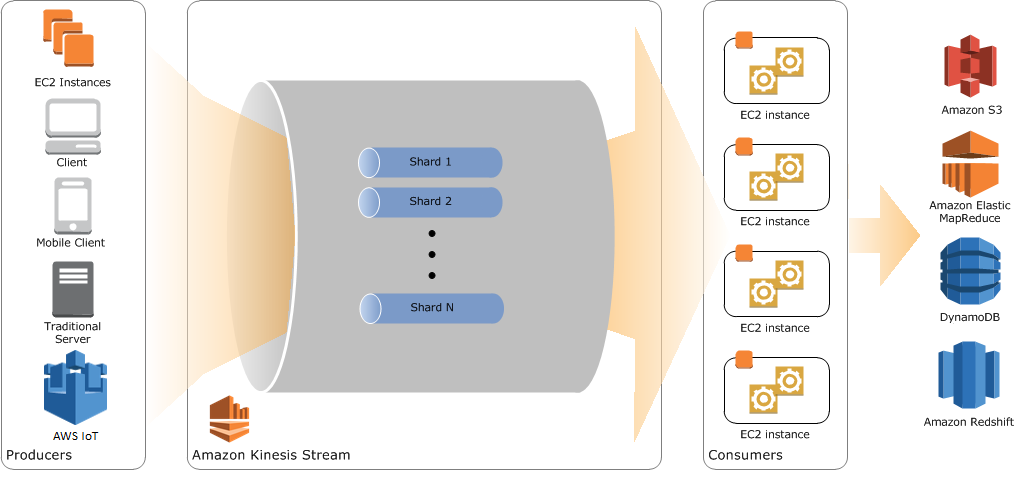
\includegraphics[scale=0.3]{images/architecture}}
\caption{Kinesis streams building blocks} \cite{www-kinesis-arch}
\label{fig:false-color}
\end{figure}

Following are key components in streams architecture \cite{www-kinesis-arch} :
\subsection{Data Record}
Its one unit of data that flows through Kinesis stream. Data records is made up of sequence number, partition key, and blob of actual data. Size of data blob is max 1 MB. During aggregation one more records are aggregated in to a single aggregated record. Further these aggregated records are emitted as an aggregation collection.

\begin{figure}[htbp]
\centering
\fbox{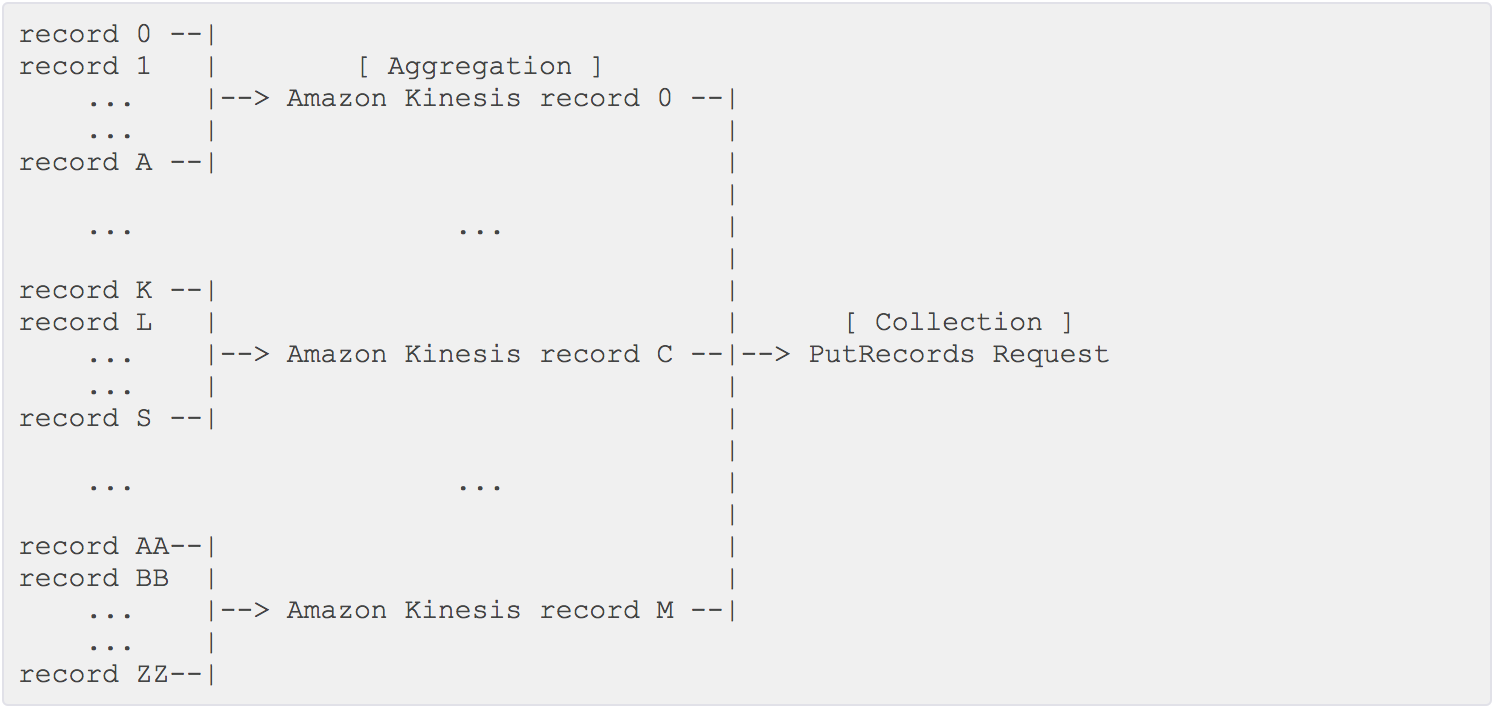
\includegraphics[scale=0.3]{images/records}}
\caption{Aggregation of records}
\label{fig:false-color}
\end{figure}

\subsection{Producer}
Producers write the data to Kinesis stream. Producer can be any system producing data for example ad server, social media stream, log server etc,

\subsection{Consumer}
 Consumers subscribe to one or more streams.  Consumer can be one of the application  running on aws or hosted on EC2.
 
\subsection{Consumer}
A stream can have one or more shards. Records are processed by each shard based on the partition key. Each shard can process upto 2MB/s data for reads and upto 1MB/s for writes. Total capacity of a stream is sum of capacities of its shards.

\subsection{Partition Keys} 
Partition key is 256 bytes long. A MD5 hash function is used to map partition keys to 128 bit integer values which is further used to map to appropriate shard.

\subsection{Sequence Number}
Sequence number is assigned to a record when a record get written to the stream. 

\subsection{Amazon Kinesis Client Library}
Amazon Kinesis Client Library is bundled into your application built on AWS. It makes sure for each record there is a shard available to process that record. Client library uses dynamo db to store control data records being processed by shards.

\subsection{Application Name}
Name of application in the control table in dynamodb where kinesis streams will write the data to. This name is unique.

\section{Creating Streams}

You can create a stream using following ways:
\begin{itemize}
	\item kinesis console
	\item Streams API
	\item AWS CLI
\end{itemize}

Before creating stream you should determine initial size of the stream \cite{www-kinesis-size} and number of shards required to create your stream. Number of shards can be calculated using the following formulae
\begin{multline*} 
number_of_shards = \\
   max ( 
   incomingWriteBandwidthInKB/1000, \\
   outgoingReadBandwidthInKB/2000
   )
\end{multline*}

Here, the attributes used in the calculation are self explanatory.

Producer for streams writes data records into Kinesis streams. This data is available for 24 hours within streams. The default retention interval can be changed. To write records to stream, you must specify partition key, name of stream and data blob. Consumer on the other hand reads data from streams using shard iterator. Shard iterator provides consumer a position on streams from where the consumer can start reading the data.

\section{Stream Limits}
\subsection{Shard}
By default there can 25 shards in a region except US east, EU and US west which has limit of 50 shards. Each shard can support up to 5 transactions per second for reads and maximum data rate of 2 MB per second. Each shard can support 1000 records per second for writes and maximum data rate of 1MB per second.

\subsection{Data retention}
By default the data is available for 24 hours which can be configured up to 168 hours with 1 hour increments.

\subsection{Data Blob}
Maximum size of data blob is 1MB before base64 encoding.

\section{Management}
Kinesis provides all management using:
\begin{itemize}
	\item  AWS console
	\item Java SDK \cite{www-kinesis-javasdk} 
\end{itemize}

\subsection{Java SDK}
AWS provides a java SDK. Java SDK \cite{www-kinesis-javasdk} can be used to complete all workflow on stream. Workflow like create, listing, retrieving shards from stream, deleting stream, resharding stream and changing data retention period. SDK provide rich documentation and developer blogs to support development on streams.

\subsection{AWS console}
AWS provides a web console to manage all AWS services including kinesis.  Using console web user interface user can perform all operations to manage stream.

\section{Monitoring}
AWS provides several ways to monitor streams. These are:
\begin{itemize}
	\item  CloudWatch metrics
	\item Kinesis Agent 
	\item API logging
	\item Client library
	\item Producer Library 
\end{itemize}

Using CloudWatch metrics allows you can monitor the data and usage at shard level.  It can collect metrics like: latency, coming bytes, incoming records, success count etc.

\section{Licensing}
Kinesis is software as a service(SAAS) from Amazon AWS infrastructure. Hence it can only run as a service within AWS. It comes with pay as you go pricing.

\section{Use Cases}

Kinesis streams and firehose can be useful in variety of use cases \cite{www-kinesis} 
\begin{itemize}
	\item  log data processing
	\item log mining
	\item realtime metrics and reporting
	\item realtime analytics
	\item complex stream processing
\end{itemize}

Kinesis solves variety of these business problems by doing a real time analysis and aggregation. This aggregated data can further be stored or available to query. Since it runs on amazon, it becomes easy for users to integrate and use other AWS components.

\section{Conclusion}
Kinesis can process huge amounts of data in realtime. Application developers can then focus on business logic. Kinesis \cite{varia2014overview} an help build realtime dashboards, capture anomalies, generate alerts, provide recommendations which can help take business and operation decisions in real time. It can also send data to other AWS services like S3, dynamodb, redshift etc. You can scale up or scale down as you demand increases or decreases and pay based on your usage. Only downside of Kinesis it that it cannot run on a private or hybrid cloud rather can only on AWS public cloud or Amazon VPC(Virtual Private Cloud). Customers who want to use Kinesis but don't want to be on Amazon platform cannot use it. Its comparable with open source Apache Kafka\cite{deyhim2016kafka} . However, Kafka lacks in high availability and monitoring in case of cloud deployments. 

\section*{Acknowledgements}
Special thanks to Professor Gregor von Laszewski, Dimitar Nikolov and all associate instructors for all help and guidance related to latex and bibtex, scripts for building the project, quick and timely resolution to any technical issues faced. The paper is written during the course  {I524: Big Data and Open Source Software Projects, Spring 2017} at Indiana University Bloomington.

 
\medskip

% Bibliography
% \bibliographystyle{unsrt}
\bibliography{references}

\end{document}
